% AUTO-GENERATED by generate_figures.py -- do not edit by hand.
% Re-run generate_figures.py after run_tests.py to update charts.

% ── Figure 1: Relative improvement over baseline (all instances) ─────────
\begin{figure}[H]
\centering
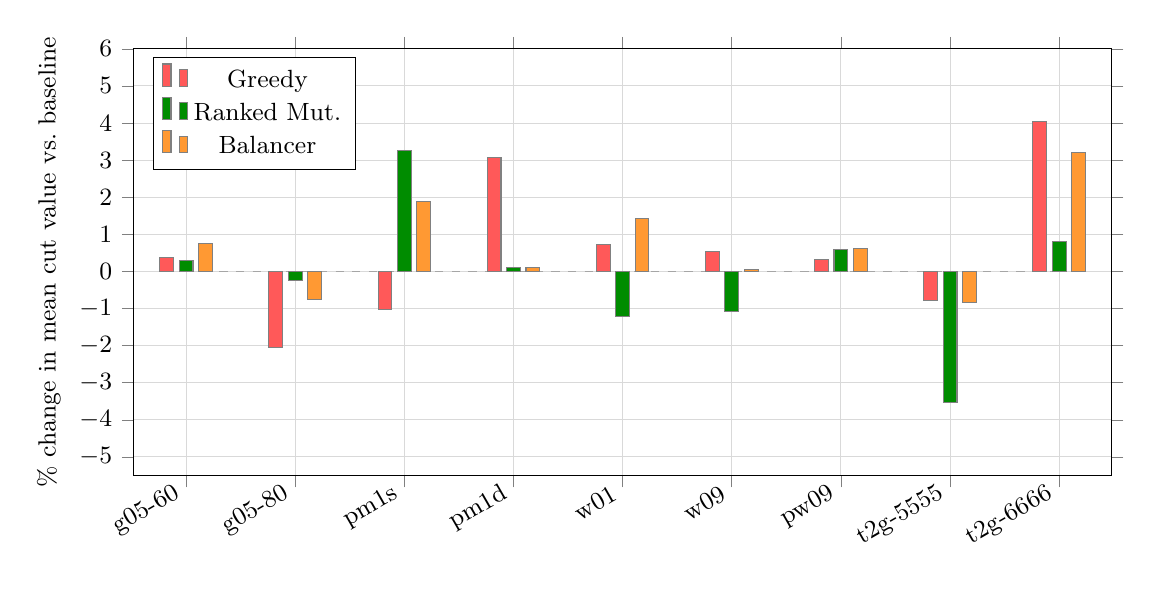
\begin{tikzpicture}
\begin{axis}[
    ybar,
    width=14cm, height=7cm,
    bar width=5pt,
    symbolic x coords={{g05-60}, {g05-80}, {pm1s}, {pm1d}, {w01}, {w09}, {pw09}, {t2g-5555}, {t2g-6666}},
    xtick=data,
    xticklabel style={rotate=30,anchor=east,font=\small},
    yticklabel style={font=\small},
    ylabel={\% change in mean cut value vs.\ baseline},
    ylabel style={font=\small},
    ymin=-5.5, ymax=6,
    ytick={-5,-4,-3,-2,-1,0,1,2,3,4,5,6},
    legend style={at={(0.02,0.98)},anchor=north west,font=\small},
    grid=both, grid style={line width=0.3pt,draw=gray!30},
    enlarge x limits=0.06, tick align=outside,
]
\draw[black!35,dashed] (axis cs:{g05-60},0) -- (axis cs:{t2g-6666},0);
    \addplot[fill=red!65,draw=black!50]
        coordinates { ({g05-60},0.381) ({g05-80},-2.056) ({pm1s},-1.026) ({pm1d},3.063) ({w01},0.714) ({w09},0.529) ({pw09},0.321) ({t2g-5555},-0.788) ({t2g-6666},4.046) };
    \addlegendentry{Greedy}
    \addplot[fill=green!55!black,draw=black!50]
        coordinates { ({g05-60},0.305) ({g05-80},-0.236) ({pm1s},3.248) ({pm1d},0.107) ({w01},-1.221) ({w09},-1.089) ({pw09},0.589) ({t2g-5555},-3.542) ({t2g-6666},0.805) };
    \addlegendentry{Ranked Mut.}
    \addplot[fill=orange!80,draw=black!50]
        coordinates { ({g05-60},0.763) ({g05-80},-0.750) ({pm1s},1.880) ({pm1d},0.107) ({w01},1.429) ({w09},0.042) ({pw09},0.616) ({t2g-5555},-0.850) ({t2g-6666},3.211) };
    \addlegendentry{Balancer}
\end{axis}
\end{tikzpicture}
\caption{Relative change in mean cut value compared to the baseline GA
          (no heuristics), across all nine benchmark instances.
          Positive values indicate improvement over the baseline.
          Each bar is the mean over five independent runs.}
\label{fig:relative-improvement}
\end{figure}

% ── Figure 2: Primary instances — all configs with stdev ─────────────────
\begin{figure}[H]
\centering
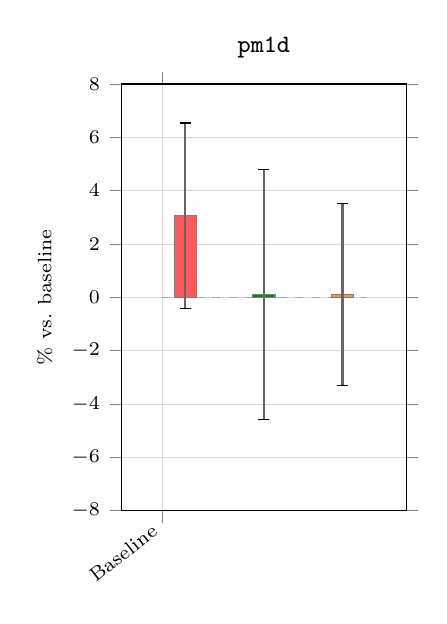
\begin{tikzpicture}
\begin{axis}[
    ybar,
    title={\texttt{pm1d}},
    title style={font=\small\ttfamily},
    width=5.2cm, height=7.0cm, bar width=8pt,
    symbolic x coords={{Baseline}, {Greedy}, {Ranked}, {Balancer}, {All}},
    xtick=data,
    xticklabel style={rotate=38,anchor=east,font=\scriptsize},
    yticklabel style={font=\scriptsize},
    ylabel={\% vs.\ baseline}, ylabel style={font=\scriptsize},
    ymin=-8, ymax=8,
    ytick={-8,-6,-4,-2,0,2,4,6,8},
    grid=both, grid style={line width=0.3pt,draw=gray!30},
    enlarge x limits=0.2, tick align=outside,
]
\draw[black!35,dashed] (axis cs:{Baseline},0) -- (axis cs:{All},0);
    \addplot[fill=blue!55,draw=black!50,
        error bars/.cd,y dir=both,y explicit,
        error bar style={draw=black!60,line width=0.8pt}]
        coordinates { ({Baseline},0.000) +- (0,4.973) };
    \addplot[fill=red!65,draw=black!50,
        error bars/.cd,y dir=both,y explicit,
        error bar style={draw=black!60,line width=0.8pt}]
        coordinates { ({Greedy},3.063) +- (0,3.474) };
    \addplot[fill=green!55!black,draw=black!50,
        error bars/.cd,y dir=both,y explicit,
        error bar style={draw=black!60,line width=0.8pt}]
        coordinates { ({Ranked},0.107) +- (0,4.686) };
    \addplot[fill=orange!80,draw=black!50,
        error bars/.cd,y dir=both,y explicit,
        error bar style={draw=black!60,line width=0.8pt}]
        coordinates { ({Balancer},0.107) +- (0,3.428) };
    \addplot[fill=violet!70,draw=black!50,
        error bars/.cd,y dir=both,y explicit,
        error bar style={draw=black!60,line width=0.8pt}]
        coordinates { ({All},-1.612) +- (0,4.361) };
\end{axis}
\end{tikzpicture}
\hspace{0.4cm}
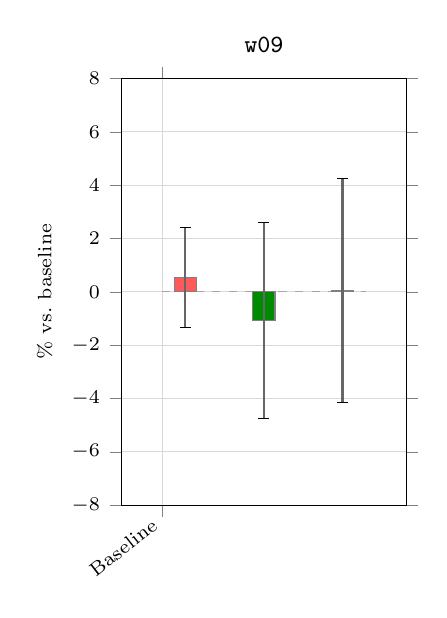
\begin{tikzpicture}
\begin{axis}[
    ybar,
    title={\texttt{w09}},
    title style={font=\small\ttfamily},
    width=5.2cm, height=7.0cm, bar width=8pt,
    symbolic x coords={{Baseline}, {Greedy}, {Ranked}, {Balancer}, {All}},
    xtick=data,
    xticklabel style={rotate=38,anchor=east,font=\scriptsize},
    yticklabel style={font=\scriptsize},
    ylabel={\% vs.\ baseline}, ylabel style={font=\scriptsize},
    ymin=-8, ymax=8,
    ytick={-8,-6,-4,-2,0,2,4,6,8},
    grid=both, grid style={line width=0.3pt,draw=gray!30},
    enlarge x limits=0.2, tick align=outside,
]
\draw[black!35,dashed] (axis cs:{Baseline},0) -- (axis cs:{All},0);
    \addplot[fill=blue!55,draw=black!50,
        error bars/.cd,y dir=both,y explicit,
        error bar style={draw=black!60,line width=0.8pt}]
        coordinates { ({Baseline},0.000) +- (0,3.729) };
    \addplot[fill=red!65,draw=black!50,
        error bars/.cd,y dir=both,y explicit,
        error bar style={draw=black!60,line width=0.8pt}]
        coordinates { ({Greedy},0.529) +- (0,1.883) };
    \addplot[fill=green!55!black,draw=black!50,
        error bars/.cd,y dir=both,y explicit,
        error bar style={draw=black!60,line width=0.8pt}]
        coordinates { ({Ranked},-1.089) +- (0,3.674) };
    \addplot[fill=orange!80,draw=black!50,
        error bars/.cd,y dir=both,y explicit,
        error bar style={draw=black!60,line width=0.8pt}]
        coordinates { ({Balancer},0.042) +- (0,4.192) };
    \addplot[fill=violet!70,draw=black!50,
        error bars/.cd,y dir=both,y explicit,
        error bar style={draw=black!60,line width=0.8pt}]
        coordinates { ({All},-0.323) +- (0,2.952) };
\end{axis}
\end{tikzpicture}
\hspace{0.4cm}
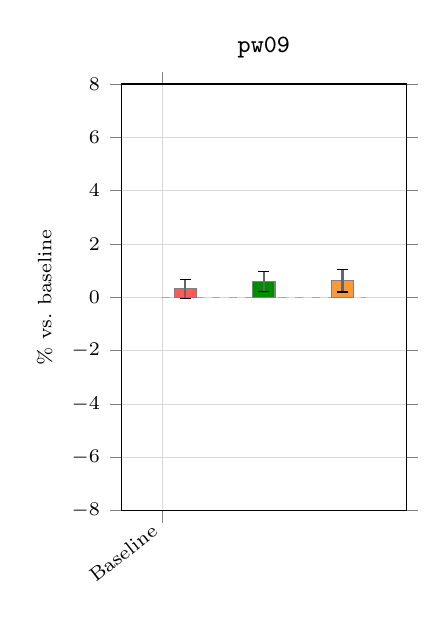
\begin{tikzpicture}
\begin{axis}[
    ybar,
    title={\texttt{pw09}},
    title style={font=\small\ttfamily},
    width=5.2cm, height=7.0cm, bar width=8pt,
    symbolic x coords={{Baseline}, {Greedy}, {Ranked}, {Balancer}, {All}},
    xtick=data,
    xticklabel style={rotate=38,anchor=east,font=\scriptsize},
    yticklabel style={font=\scriptsize},
    ylabel={\% vs.\ baseline}, ylabel style={font=\scriptsize},
    ymin=-8, ymax=8,
    ytick={-8,-6,-4,-2,0,2,4,6,8},
    grid=both, grid style={line width=0.3pt,draw=gray!30},
    enlarge x limits=0.2, tick align=outside,
]
\draw[black!35,dashed] (axis cs:{Baseline},0) -- (axis cs:{All},0);
    \addplot[fill=blue!55,draw=black!50,
        error bars/.cd,y dir=both,y explicit,
        error bar style={draw=black!60,line width=0.8pt}]
        coordinates { ({Baseline},0.000) +- (0,0.163) };
    \addplot[fill=red!65,draw=black!50,
        error bars/.cd,y dir=both,y explicit,
        error bar style={draw=black!60,line width=0.8pt}]
        coordinates { ({Greedy},0.321) +- (0,0.365) };
    \addplot[fill=green!55!black,draw=black!50,
        error bars/.cd,y dir=both,y explicit,
        error bar style={draw=black!60,line width=0.8pt}]
        coordinates { ({Ranked},0.589) +- (0,0.383) };
    \addplot[fill=orange!80,draw=black!50,
        error bars/.cd,y dir=both,y explicit,
        error bar style={draw=black!60,line width=0.8pt}]
        coordinates { ({Balancer},0.616) +- (0,0.416) };
    \addplot[fill=violet!70,draw=black!50,
        error bars/.cd,y dir=both,y explicit,
        error bar style={draw=black!60,line width=0.8pt}]
        coordinates { ({All},0.017) +- (0,0.323) };
\end{axis}
\end{tikzpicture}
\caption{Mean cut value relative to the baseline (\%) for the three primary
          benchmark instances (\texttt{pm1d\_100.9}, \texttt{w09\_100.9},
          \texttt{pw09\_100.9}). Error bars show $\pm 1$ standard deviation
          over the repeated runs. The dashed line marks zero (baseline level).
          The \emph{All Three} bar corresponds to 10 runs; all others to 5.}
\label{fig:primary-instances}
\end{figure}

% ── Figure 3: Wall-clock time overhead ───────────────────────────────────
\begin{figure}[H]
\centering
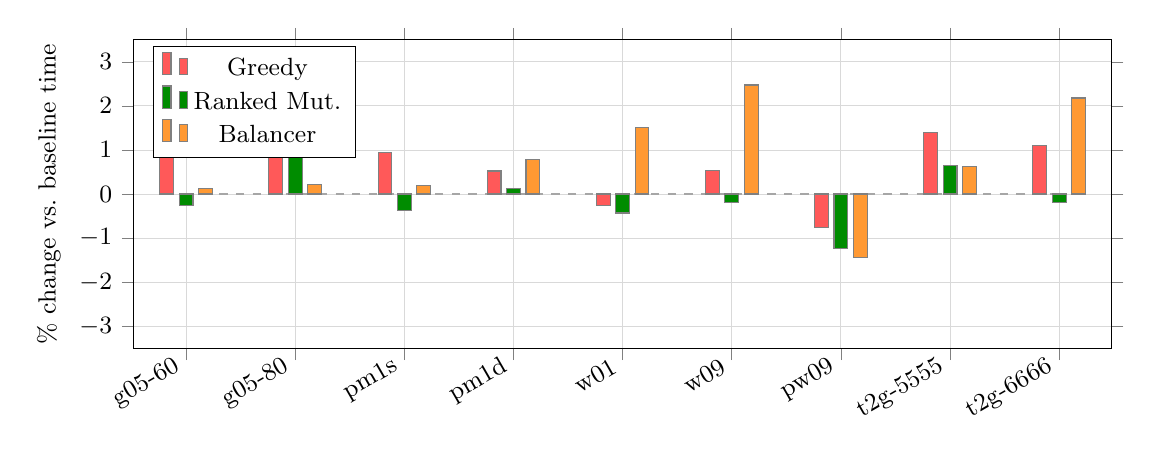
\begin{tikzpicture}
\begin{axis}[
    ybar,
    width=14cm, height=5.5cm,
    bar width=5pt,
    symbolic x coords={{g05-60}, {g05-80}, {pm1s}, {pm1d}, {w01}, {w09}, {pw09}, {t2g-5555}, {t2g-6666}},
    xtick=data,
    xticklabel style={rotate=30,anchor=east,font=\small},
    yticklabel style={font=\small},
    ylabel={\% change vs.\ baseline time},
    ylabel style={font=\small},
    ymin=-3.5, ymax=3.5,
    ytick={-3,-2,-1,0,1,2,3},
    legend style={at={(0.02,0.98)},anchor=north west,font=\small},
    grid=both, grid style={line width=0.3pt,draw=gray!30},
    enlarge x limits=0.06, tick align=outside,
]
\draw[black!35,dashed] (axis cs:{g05-60},0) -- (axis cs:{t2g-6666},0);
    \addplot[fill=red!65,draw=black!50]
        coordinates { ({g05-60},1.229) ({g05-80},1.286) ({pm1s},0.944) ({pm1d},0.522) ({w01},-0.253) ({w09},0.539) ({pw09},-0.767) ({t2g-5555},1.394) ({t2g-6666},1.094) };
    \addlegendentry{Greedy}
    \addplot[fill=green!55!black,draw=black!50]
        coordinates { ({g05-60},-0.254) ({g05-80},1.575) ({pm1s},-0.364) ({pm1d},0.126) ({w01},-0.431) ({w09},-0.195) ({pw09},-1.242) ({t2g-5555},0.651) ({t2g-6666},-0.200) };
    \addlegendentry{Ranked Mut.}
    \addplot[fill=orange!80,draw=black!50]
        coordinates { ({g05-60},0.116) ({g05-80},0.213) ({pm1s},0.203) ({pm1d},0.789) ({w01},1.514) ({w09},2.474) ({pw09},-1.432) ({t2g-5555},0.618) ({t2g-6666},2.178) };
    \addlegendentry{Balancer}
\end{axis}
\end{tikzpicture}
\caption{Wall-clock execution time of the evolutionary loop relative to
          the baseline (\%), per instance and heuristic.
          All deviations are within $\pm 3\%$, confirming that the
          heuristic operators introduce negligible computational overhead.}
\label{fig:timing}
\end{figure}
